\section{Результаты тестирования}
\label{sec:Chapter6} \index{Chapter6}

\subsection{Датасеты}

В качестве множества $A$ будем рассматривать датасет CIFAR-10 \cite{cifar10}. Он состоит из 60.000 цветных изображений размером 32$\times$32. Изображения разделены на 10 классов. В каждом классе содержится 5000 изображений для обучения и 1000 для тестирования. Таким образом, обучающая и тестовая выборка составляют 50.000 и 10.000 изображений соответственно.

В качестве множества $B$ будем рассматривать датасет Tiny ImageNet \cite{tiny_imagenet}. Он состоит из 120.000 цветных изображений размером 64$\times$64. Данный датасет больше предыдущего, и в нем изображения разделены на 200 классов. В каждом классе содержится 500 изображений для обучения, 50 для валидации и 50 для тестирования. Таким образом, обучающая и тестовая выборка составляют 100.000 и 10.000 изображений соответственно.

\subsection{Обучение с учителем}
\label{sabsec:supervised}

В первую очередь было проверено, какую точность классификации изображений можно получить, если использовать выбранные архитектуры для классического обучения с учителем. 

В каждую архитектуру был добавлен последний линейный слой классификации, после чего проводилось обучение.

Обе архитектуры обучались на 30 эпохах с размером пакета 256. Для обучения использовались оптимизатор SGD и функция ошибки CrossEntropyLoss.

На рисунках \ref{Arch_1_supervised} и \ref{Arch_2_supervised} изображены зависимости функции ошибки от количества итераций для архитектуры $N_1$ и $N_2$ соответственно. 

\begin{figure}[H]
    \begin{minipage}[h]{0.48\linewidth}
        \center{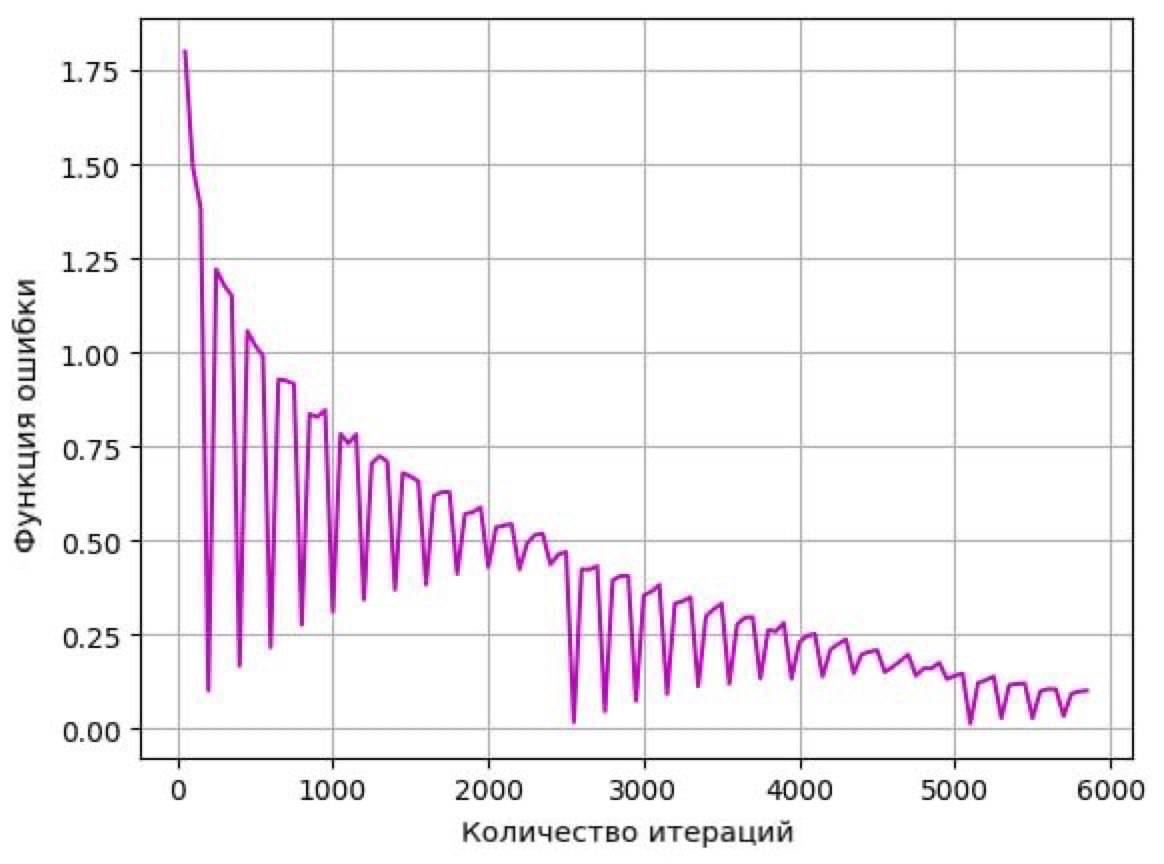
\includegraphics[width=1\linewidth]{pictures/Arch_1_supervised.jpg}} \\
        \caption{Архитектура $N_1$}
        \label{Arch_1_supervised}
    \end{minipage}
    \hfill
    \begin{minipage}[h]{0.48\linewidth}
        \center{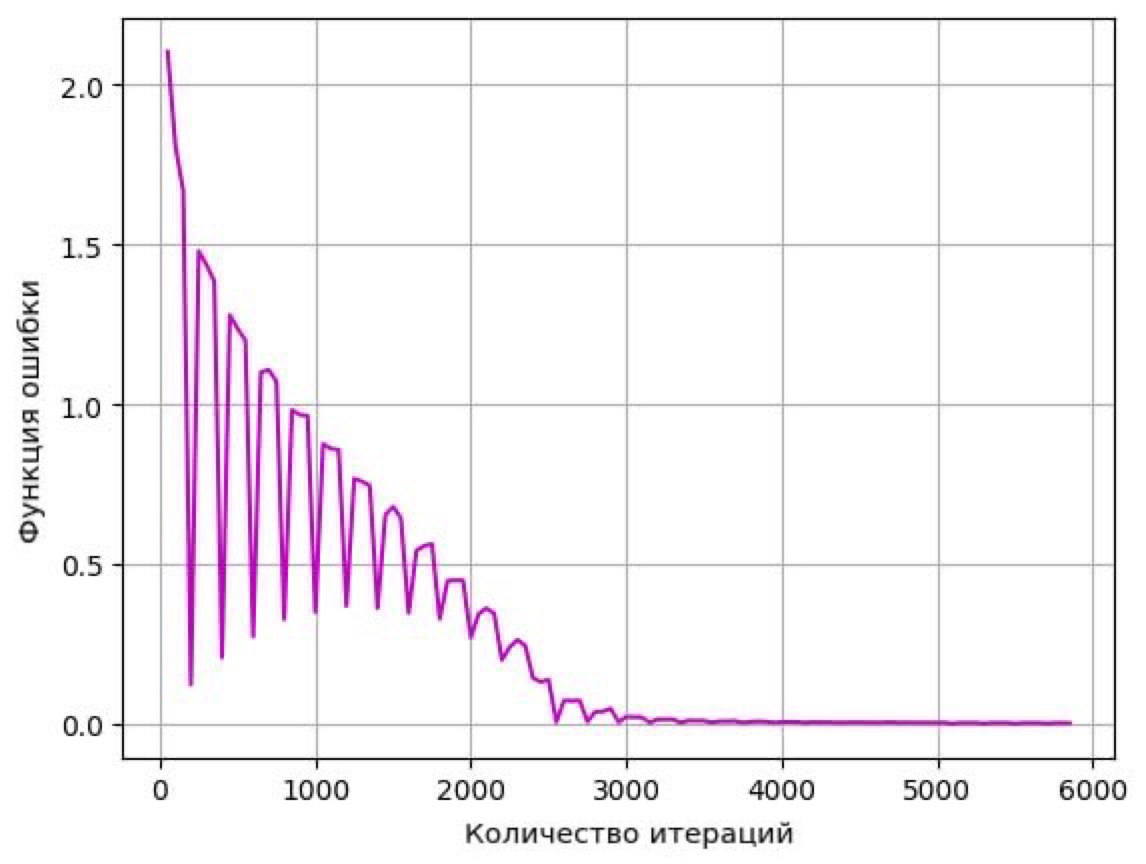
\includegraphics[width=1\linewidth]{pictures/Arch_2_supervised.jpg}} \\
        \caption{Архитектура $N_2$}
        \label{Arch_2_supervised}
    \end{minipage}
\end{figure}

Для архитектуры $N_1$ точность Top-1 и Top-5 составили 70.6\% и 97.6\% соответственно. Для архитектуры $N_2$ результаты получились хуже на 2.5\%: точность Top-1 и Top-5 составили 68.1\% и 96.5\% соответственно.

\subsection{Обучение с помощью метода VICReg}

Поскольку изображения в датасете CIFAR-10 небольшие, было принято решение перед обучением использовать следующие аугментации для обработки тренировочного набора:
\begin{itemize}
    \item RandomResizedCrop(32);
    \item RandomHorizontalFlip(p=0.5).
\end{itemize}

Далее для обеих архитектур обучение проводилось на разном количестве эпох. Было попробовано 20, 30 и 40 эпох. Размер пакета для всех случаев составлял 256. Оптимальным оказалось 30 эпох, так как меньшего количества не хватало для хороших результатов точности, а при большем количестве начиналось переобучение.

Для регуляризации компонент функции потерь использовались значения 25, 25, 1 для дисперсии, инвариантности и ковариации соответственно.

На рисунках \ref{Arch_1_vicreg} и \ref{Arch_2_vicreg} изображены зависимости функции ошибки от количества итераций на 30 эпохах для архитектуры $N_1$ и $N_2$ соответственно.

\begin{figure}[H]
    \begin{minipage}[h]{0.48\linewidth}
        \center{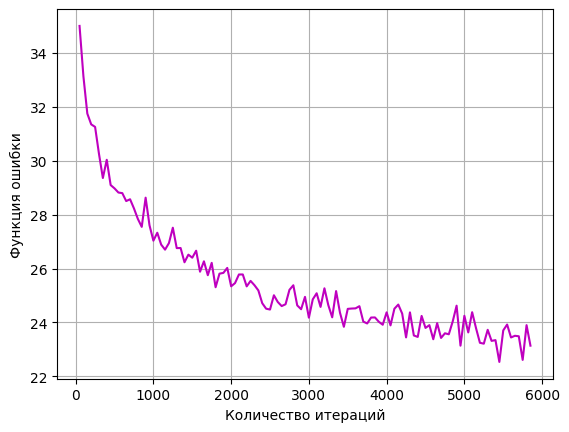
\includegraphics[width=1\linewidth]{pictures/Arch_1_vicreg.png}} \\
        \caption{Архитектура $N_1$}
        \label{Arch_1_vicreg}
    \end{minipage}
    \hfill
    \begin{minipage}[h]{0.48\linewidth}
        \center{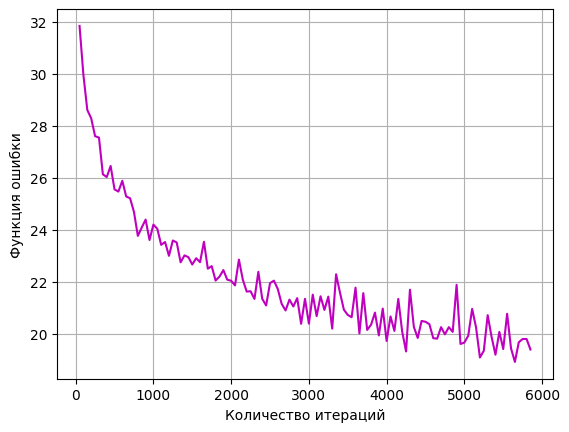
\includegraphics[width=1\linewidth]{pictures/Arch_2_vicreg.png}} \\
        \caption{Архитектура $N_2$}
        \label{Arch_2_vicreg}
    \end{minipage}
\end{figure}

Также для наглядности к полученным после обучения эмбедингам был применен метод T-SNE \cite{TSNE}. 

На рисунке \ref{TSNE_first} изображена проекция на двумерную плоскость изначальной выборки.

\begin{figure}[H]
    \center{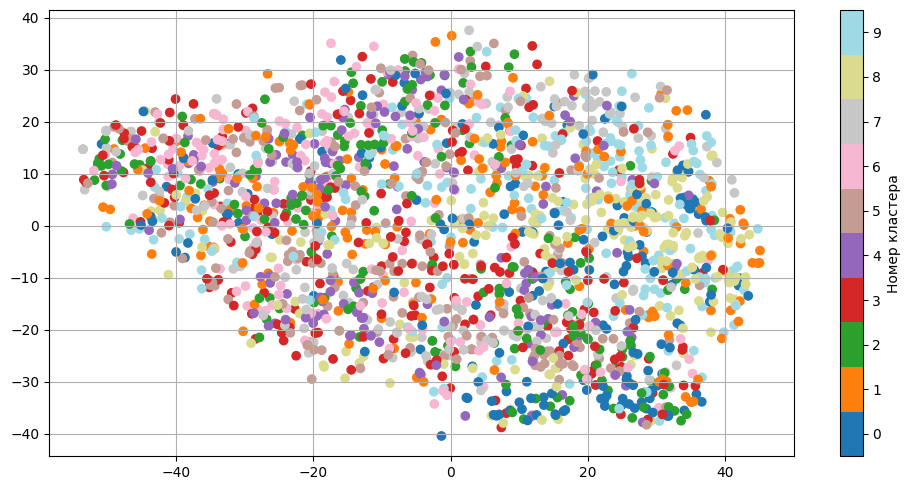
\includegraphics[height=7.5cm, keepaspectratio]{pictures/TSNE_first.png}}
        \caption{Применение метода T-SNE для изначальной выборки}
        \label{TSNE_first}
\end{figure} 

На рисунках \ref{TSNE_arch_1} и \ref{TSNE_arch_2} изображены отображения для эмбедингов, полученных с помощью архитектуры $N_1$ и $N_2$ соответственно

\begin{figure}[H]
    \begin{minipage}[h]{0.5\linewidth}
        \center{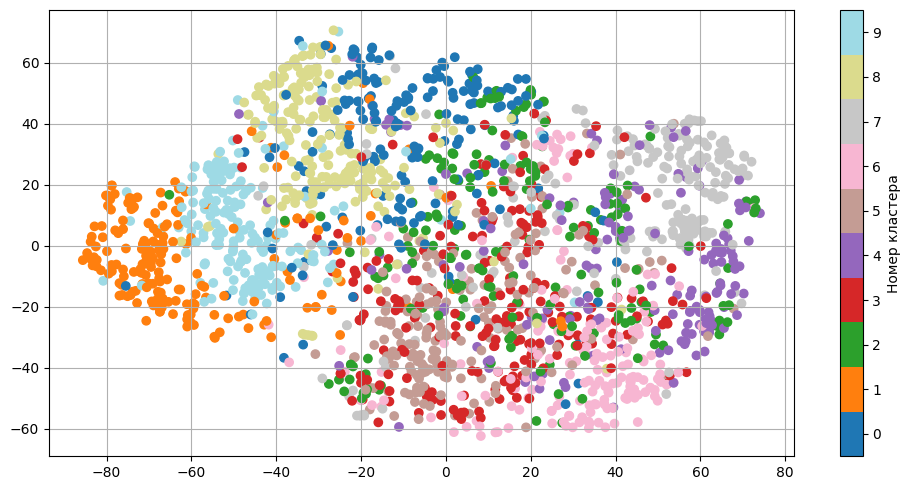
\includegraphics[width=1\linewidth]{pictures/TSNE_arch_1.png}} \\
        \caption{Архитектура $N_1$}
        \label{TSNE_arch_1}
    \end{minipage}
    \hfill
    \begin{minipage}[h]{0.5\linewidth}
        \center{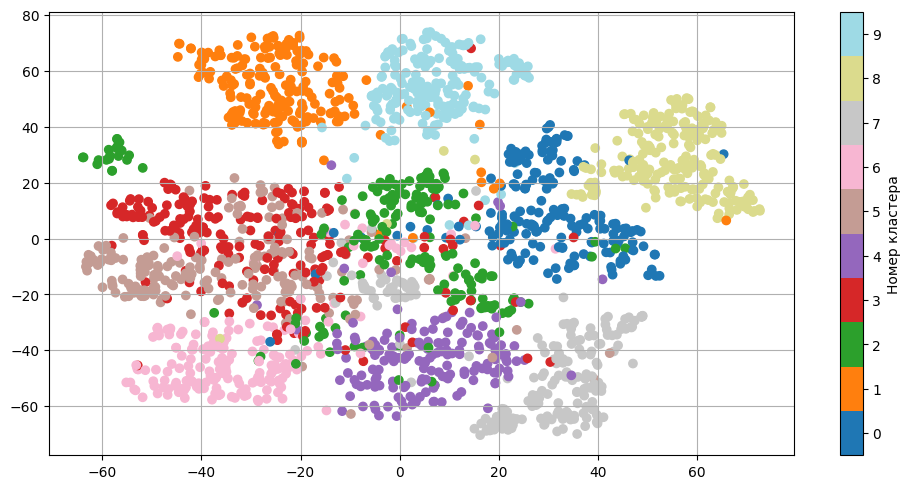
\includegraphics[width=1\linewidth]{pictures/TSNE_arch_2.png}} \\
        \caption{Архитектура $N_2$}
        \label{TSNE_arch_2}
    \end{minipage}
\end{figure}

\subsection{Результаты}

Тестирование проводилось на 20 эпохах с размером пакета 256. В таблице ниже приведены результаты точности из раздела \ref{sabsec:supervised}, полученные после обучения с учителем, и результаты точности, полученные с помощью метода VICReg на наборе CIFAR-10.


\begin{center}
\begin{tabular}{ l c c c c c } 
  \hline
  \multirow{3}{4em}{Метод} & \multicolumn{2}{c}{Архитектура $N_1$} & & \multicolumn{2}{c}{Архитектура $N_2$} \\
  \cline{2-3}\cline{5-6}

  & \multicolumn{2}{c}{Точность} & & \multicolumn{2}{c}{Точность} \\
  & Top-1 & Top-5 & &  Top-1 & Top-5  \\ 
  \hline

  Обучение с учителем \cite{cifar10} & 70.6 & 97.6 & & 68.1 & 96.5 \\
  VICReg \cite{tiny_imagenet} & 64.8 & 96.9 & & 89.6 & 99.7 \\

  \hline
\end{tabular}
\end{center}

Как видно из таблицы, с помощью метода VICReg удалось получить более высокую точность, чем при обучении с учителем. Но хороший результат получается только при использовании архитектуры $N_2$, которая является достаточно сложной, и имеет примерно в 29 раз больше параметров, чем архитектура $N_1$.

Для архитектуры $N_2$ было проведено тестирование на наборе Tiny ImageNet. Для тестирования также использовалось частичное обучение, которое описано в разделе \ref{Eval}. Тестирование проводилось на 20 эпохах с размером пакета 256. В таблице ниже для сравнения представлены результаты точности на наборе CIFAR-10 и на наборе Tiny ImageNet. 

\begin{center}
\begin{tabular}{ l c c c c c c c } 
  \hline
  \multirow{3}{4em}{Датасет} & \multicolumn{2}{c}{Линейная оценка} & & \multicolumn{4}{c}{Частичное обучение} \\
  \cline{2-3}\cline{5-8}
  
  & Top-1 & Top-5 & &  \multicolumn{2}{c}{Top-1} &  \multicolumn{2}{c}{Top-5}  \\ 
  & & & & 1\% & 10\% & 1\% & 10\% \\ 
  \hline

  CIFAR-10 \cite{cifar10} & 89.6 & 99.7 & & 85.5 & 90.3 & 99.2 & 99.7 \\
  Tiny ImageNet \cite{tiny_imagenet} & 52.3 & 74.0 & & 79.7 & 86.4 & 94.7 & 95.9 \\
  
  \hline
\end{tabular}
\end{center}

